\begin{figure}[tbp]
  \centering
  {\small
    Linear part: $C_0\xrightarrow{d_1}C_1\xrightarrow{d_1}C_2$,
    \quad $H_a=H^a(C_\bullet,d_1)$.\par}
  \medskip
  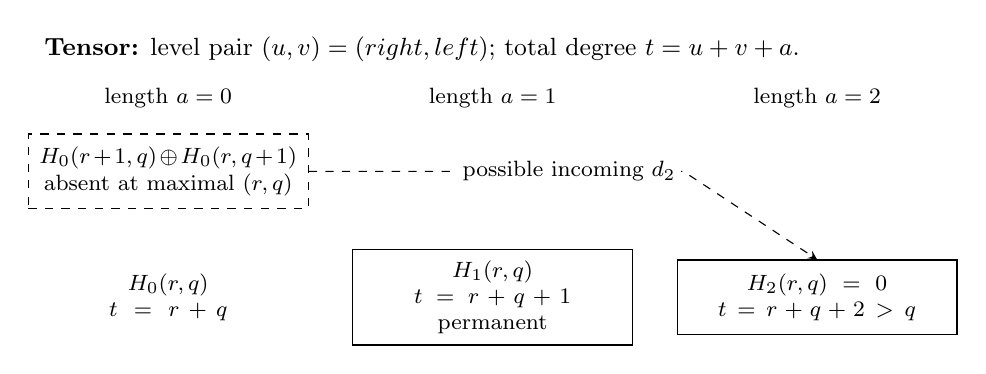
\begin{tikzpicture}[
      x=.01\linewidth,y=1cm,
      every node/.style={font=\footnotesize,align=center},
      term/.style={text width=.27\linewidth,inner sep=4pt},
      permanent/.style={term,draw,semithick,minimum height=.95cm},
      endpoint/.style={term,draw,thin,minimum height=.95cm},
      excluded/.style={term,draw,dashed,thin,minimum height=.95cm},
      differential/.style={->,thin,>=stealth}
    ]
    \node[anchor=west,align=left,font=\small] at (-14,0)
      {\textbf{Tensor:} level pair $(u,v)=(\text{right},\text{left})$;
        total degree $t=u+v+a$.};
    \node at (0,-.62) {length $a=0$};
    \node at (34,-.62) {length $a=1$};
    \node at (68,-.62) {length $a=2$};
    \node[excluded] (tensor-sources) at (0,-1.55)
      {$H_0(r+1,q)\oplus H_0(r,q+1)$\\
        absent at maximal $(r,q)$};
    \node[term] (tensor-zero) at (0,-3.15)
      {$H_0(r,q)$\\$t=r+q$};
    \node[permanent] (tensor-middle) at (34,-3.15)
      {$H_1(r,q)$\\$t=r+q+1$\\permanent};
    \node[endpoint] (tensor-two) at (68,-3.15)
      {$H_2(r,q)=0$\\$t=r+q+2>q$};
    \draw[differential,dashed] (tensor-sources.east)
      -- (54,-1.55) -- (tensor-two.north);
    \node[fill=white,inner sep=2pt] at (42,-1.55)
      {possible incoming $d_2$};

  \end{tikzpicture}
  \caption{The tensor length filtration at the highest contributing pair
    $(r,q)$.  The right normalized level is at most $r\ge-1$, and every
    contributing left color is in $T\cup\partial T$, where the cap is $q$.
    The only possible secondary differential is $d_2:0\to2$, so the middle
    classes are permanent.  Its two possible incoming sources at $(r,q)$
    are absent; hence the length-two classes also survive.  Their actual
    degree $r+q+2>q$ forces $H_2(r,q)=0$.  A residual right simple has
    normalized level $-1$ and assigned length $1$, which preserves the
    total-degree formula.  The dashed arrow marks an excluded possibility.
    Family and bidegree indices are suppressed.}
  \label{fig:filtrations}
\end{figure}
